Jako první určíme proud \(I_d\), to uděláme dvěma způsoby, podle požadovaného \(SR\) a podle požadovaného \(GBW\) a vybereme ten větší.

Pro oba výpočty budeme potřebovat určit kompenzační kapacitu \(C_c\), kterou určíme ze zadané kapacity na výstupu jako \(C_C = 0.3 \cdot C_L = 3 [pF]\).

Podle \(SR\)
\begin{center}
    \large
    \(
        I_d = SR \cdot C_L = 10\mu \cdot 3p = 30 [\mu A]
    \)
\end{center}

Podle \(GBW\) 
\begin{center}
    \large
    \(
        I_d = GBW \cdot U_{OV} \cdot \pi \cdot C_L = 10\mu \cdot 0.2 \cdot \pi \cdot 3p =  18.84 [\mu A]
    \)
\end{center}

Proud tedy bude \(I_{d1} = 30 [\mu A]\).

Dále můžeme určit rozměry tranzistorů \(M_1\) až \(M_5\), s tím že \(I_{dM3} = 2 \cdot I_{d1} \).
Také budeme muset zvolit napětí \(U_{OV}\), která jsme s ohledem na pracovní rozsah už v minulém kroku zvolili jako\(U_{OV} = 0.2 [V]\).
Délku tranzistoru \(L\) zvolím s ohledem na parametr \(\lambda\) \(L = 2 [\mu m]\).

\begin{center}
    \large
    \(
        W_{M1} = W_{M2} = L \cdot \frac{2 \cdot I_{d1}}{KP_N \cdot U_{OV}^2} = 2\mu \cdot \frac{2 \cdot 30\mu}{200\mu 0.2^2} = 15 [\mu m]
    \)
\end{center}

\begin{center}
    \large
    \(
        W_{M3} = L \cdot \frac{2 \cdot I_{d1}}{KP_N \cdot U_{OV}^2} = 2\mu \cdot \frac{2 \cdot 60\mu}{200\mu 0.2^2} = 30 [\mu m]
    \)
\end{center}

\begin{center}
    \large
    \(
        W_{M4} = W_{M5} = L \cdot \frac{2 \cdot I_d}{KP_P \cdot U_{OV}^2} = 2\mu \cdot \frac{2 \cdot 30\mu}{50\mu 0.2^2} = 60 [\mu m]
    \)
\end{center}

Dále můžeme určit proud výstupním stupněm jako desetinásobek proudu diferenčním stupněm, tedy \(I_{dM7} = 300 [\mu A]\), z čehož můžeme určit rozměry tranzistorů \(M6\) až \(M_7\).

\begin{center}
    \large
    \(
        W_{M6} = L \cdot \frac{2 \cdot I_d}{KP_N \cdot U_{OV}^2} = 2\mu \cdot \frac{2 \cdot 300\mu}{200\mu 0.2^2} = 150 [\mu m]
    \)
\end{center}

\begin{center}
    \large
    \(
        W_{M7} = L \cdot \frac{2 \cdot I_d}{KP_P \cdot U_{OV}^2} = 2\mu \cdot \frac{2 \cdot 300\mu}{50\mu 0.2^2} = 600 [\mu m]
    \)
\end{center}

% Proud tranzistorem \(M_3\) je součtem proudu \(I_{dM1}\) a \(I_{dM2}\) a tedy \(I_{dM3} = 20 [\mu A]\) jeho šířka tedy bude dvojnásobná \(W_{M3} = 10 [\mu A]\)
Tranzistor \(M_8\) zvolíme třetinový oproti tranzistoru \(M_3\), abychom šetřili proudem, tedy \(L=2 [\mu m] W=10[\mu m]\) a zbývá určit jen rezistor \(R_1\) jako:

\begin{center}
    \Large
    \(
        R_1 = \frac{U_{CC}-(U_{OV}+U_{TH})}{I_{dM3}} = \frac{1.8 - (0.2+0.4)}{20\mu} = 60 [k\Omega]
    \)
\end{center}

\begin{figure}[h!]
    \centering
    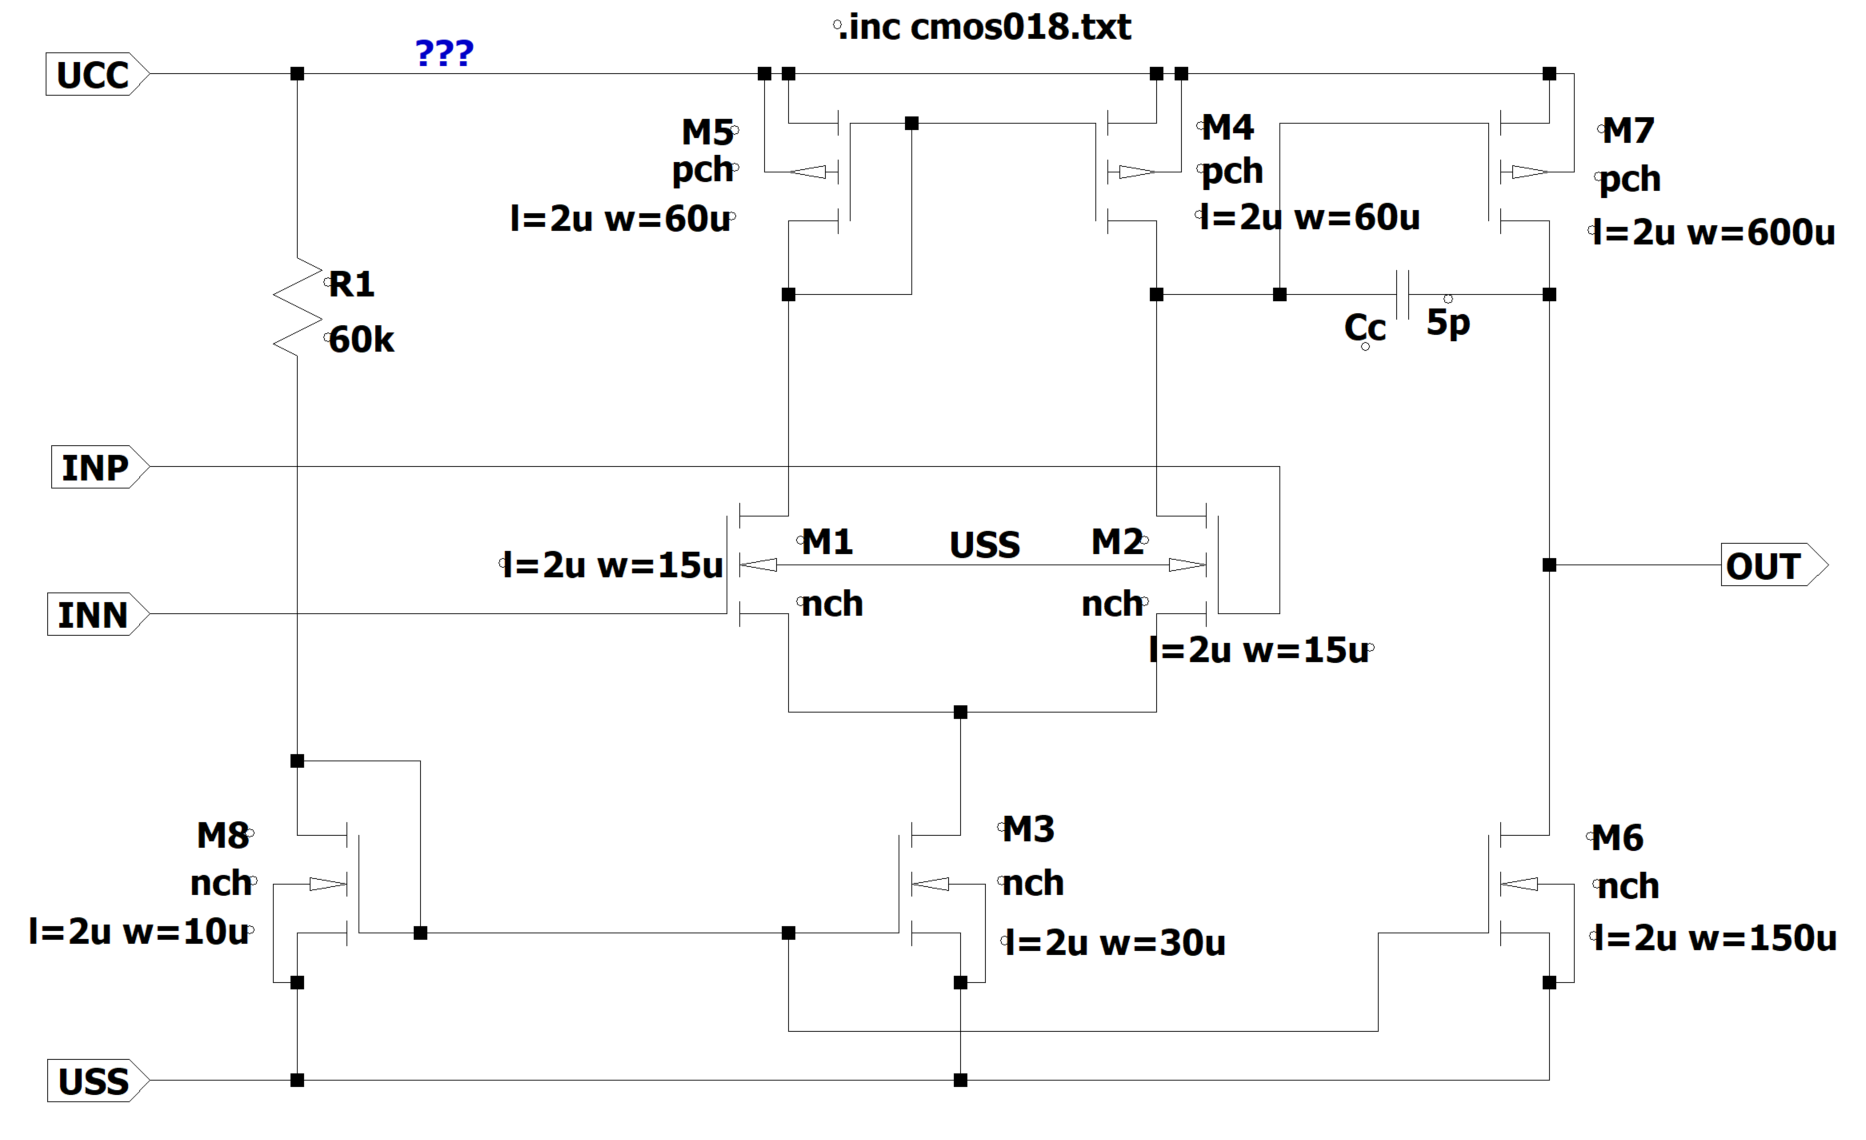
\includegraphics[width=\textwidth]{text/img/Shrnuti_sschematem.png}
    \caption{\label{fig:res-sch} Výslední schéma}
\end{figure}

Zesílení bychom mohli určit jako:
\begin{center}
    \Large
    \(
        A_{U0} = A_{1} \cdot A_{2} = 
         g_{m1} \cdot R_{01} \cdot g_{m6} \cdot R_{02} =  
        % \frac{2 \cdot I_{D1}}{U_{OV}} \frac{R_{DS1,2} \cdot R_{DS4,5}}{R_{DS1,2} + R_{DS4,5}}  \frac{2 \cdot I_{D6}}{U_{OV}} \frac{R_{DS7} \cdot R_{DS6}}{R_{DS7} + R_{DS6}} =
        \frac{2 \cdot I_{D1}}{U_{OV}} \frac{\frac{1}{\lambda_{M1,2} \cdot I_{M1,2}} \cdot \frac{1}{\lambda_{M4,5} \cdot I_{M4,5}}}{\frac{1}{\lambda_{M1,2} \cdot I_{M1,2}} + \frac{1}{\lambda_{M4,5} \cdot I_{M4,5}}}  \frac{2 \cdot I_{D6}}{U_{OV}} \frac{\frac{1}{\lambda_{M1,2} \cdot I_{M1,2}} \cdot \frac{1}{\lambda_{M7} \cdot I_{M6}}}{\frac{1}{\lambda_{M7} \cdot I_{M6}}} = 
        \frac{2 \cdot 30\mu }{0.2   } \frac{\frac{1}{0.0441692      \cdot 30\mu   } \cdot \frac{1}{0.0787698      \cdot 30\mu   }}{\frac{1}{0.0441692      \cdot 30\mu   } + \frac{1}{0.0787698      \cdot 30\mu   }}  \frac{2 \cdot 30\mu }{0.2   } \frac{\frac{1}{0.0441692      \cdot 30\mu   } \cdot \frac{1}{0.0787698    \cdot 30\mu }}{\frac{1}{0.0441692    \cdot 30\mu }} = 
        10326.438
    \)
\end{center}
V decibelech tedy:
\begin{center}
    \Large
    \(
        A_{U0-dB} = 20 \cdot log_{10}(10326.438) = 80.3 [dB]
    \)
\end{center}

Výsledné \(SR\) bychom mohli odhadnout jako:
\begin{center}
    \Large
    \(
        SR = \frac{I_{D-M7}}{C_L} = \frac{300\mu}{10p} = 30 [V/\mu s]
    \)
\end{center}

Spotřebu zesilovače jako:
\begin{center}
    \large
    \(
        P = I_{IN} \cdot U_{CC} = (I_{D-M3} + I_{D-M6} + I_{D-M8}) \cdot U_{CC} = (300\mu + 60\mu + 20\mu) \cdot 1.8 = 684 [\mu W]
    \)
\end{center}

\(GBW\) odhadneme jako:
\begin{center}
    \Large
    \(
        GBW = \frac{I_d}{U_{OV} \cdot \pi \cdot C_L} = \frac{300\mu}{0.2 \cdot \pi \cdot 10p} = 47.8 [MHz]  
    \)
\end{center}

 rozsah pak odhadneme následovně:
\begin{center}
    \large
    \(
        U_{OUT-min} = U_{OU7} = 0.2 [V] 
    \)
    \(
        U_{OUT-max} = U_{CC} - U_{OV6} = 1.8 - 0.2 = 1.6 [V]
    \)
\end{center}

\begin{center}
    \large
    \(
        U_{IN-min} = U_{GS5} + U_{OV1} - U_{GS1} = 0.6 + 0.2 - 0.6 = 0.2 [V]
    \)
    \(
        U_{IN-max} = U_{CC} - U_{GS1} - U_{OV3} = 1.8 - 0.6 - 0.2 = 1 [V]
    \)
\end{center}


\begin{figure}[h!]
    \centering
    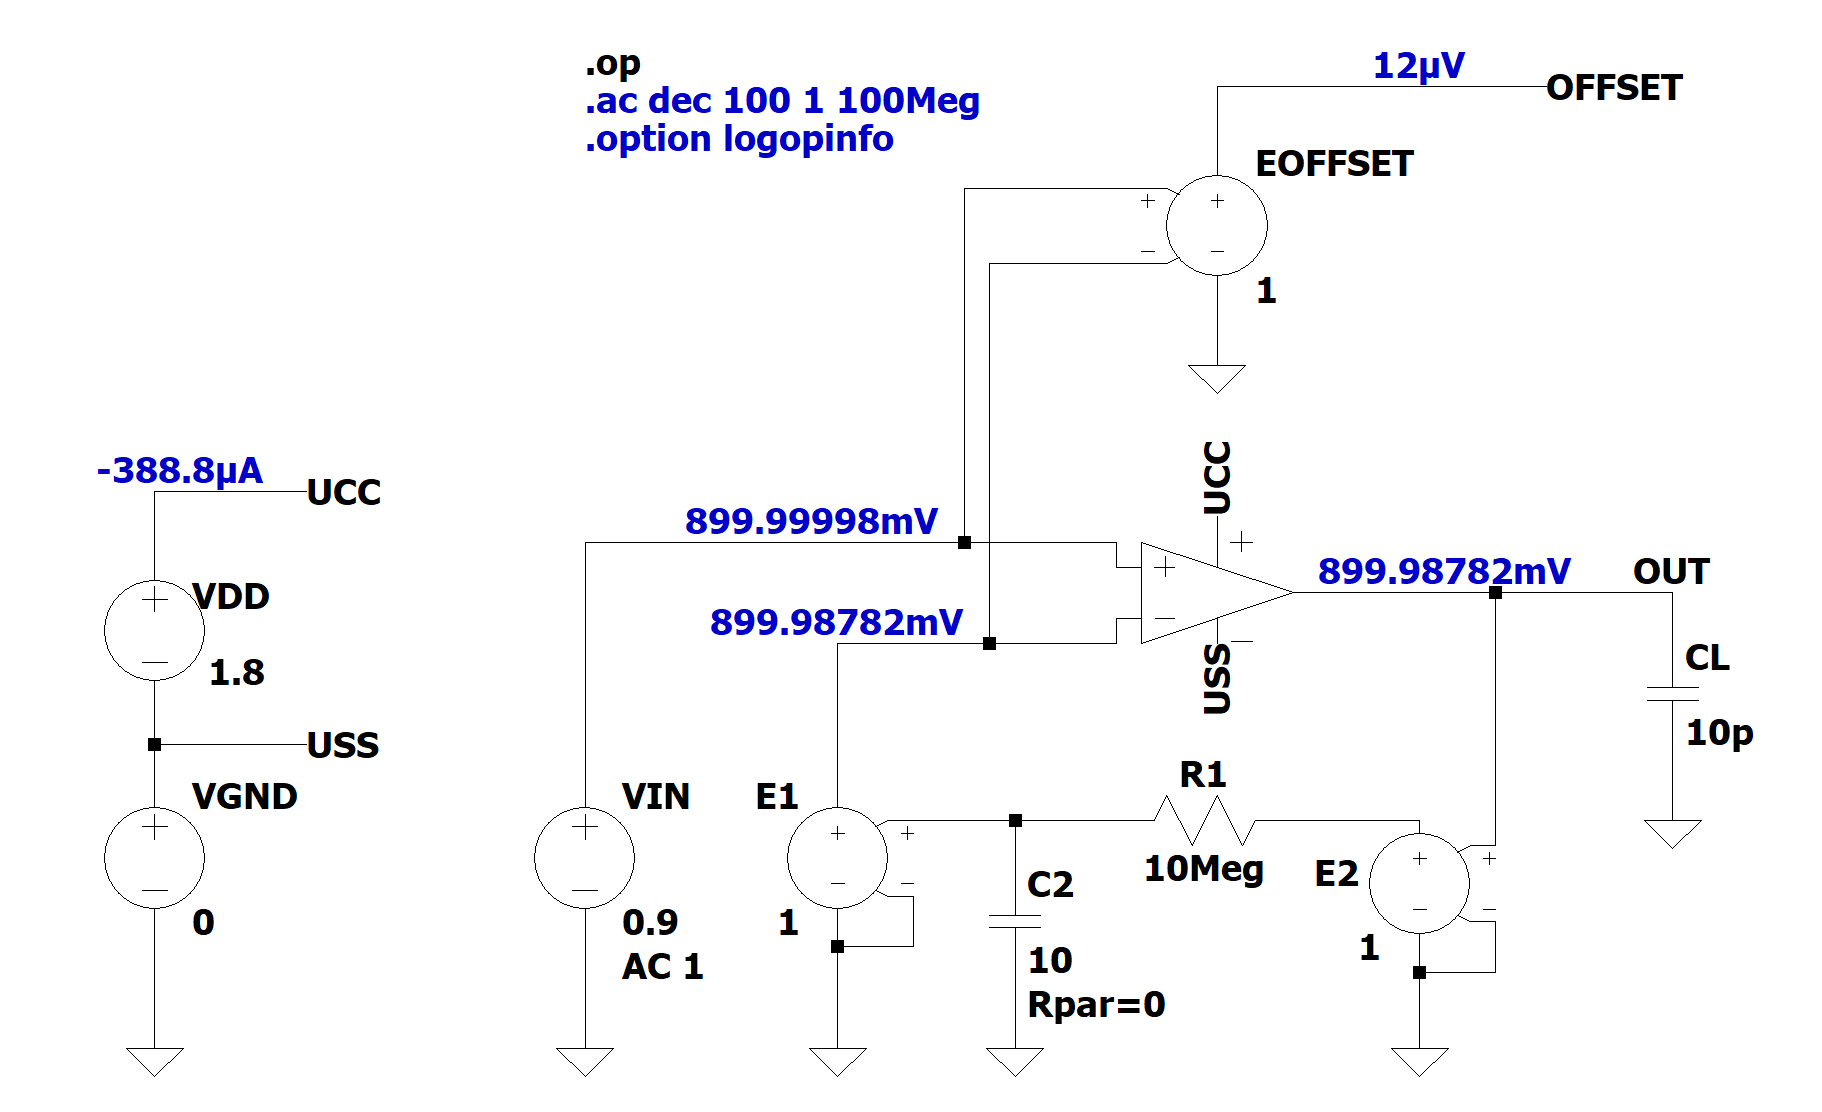
\includegraphics[width=\textwidth]{text/img/OP-sch.png}
    \caption{\label{fig:res-OP-SCH} {\bf .OP} analýza obvodu}
\end{figure}

\begin{table}[h!]
    \hspace{-13mm}
    \scriptsize
    \begin{tabular}{lcccccccc}
        \hline
        \textbf{Name:} & m1 & m2 & m3 & m6 & m8 & m4 & m5 & m7 \\
        \textbf{Model:} & nch & nch & nch & nch & nch & pch & pch & pch \\
        \hline
        Id & \(2.97\cdot10^{-5}\) & \(2.97\cdot10^{-5}\) & \(5.94\cdot10^{-5}\) & \(3.09\cdot10^{-4}\) & \(2.03\cdot10^{-5}\) & \(-2.97\cdot10^{-5}\) & \(-2.97\cdot10^{-5}\) & \(-3.09\cdot10^{-4}\) \\
        Vgs & \(6.48\cdot10^{-1}\) & \(6.48\cdot10^{-1}\) & \(5.82\cdot10^{-1}\) & \(5.82\cdot10^{-1}\) & \(5.82\cdot10^{-1}\) & \(-5.88\cdot10^{-1}\) & \(-5.88\cdot10^{-1}\) & \(-5.90\cdot10^{-1}\) \\
        Vds & \(9.59\cdot10^{-1}\) & \(9.58\cdot10^{-1}\) & \(2.52\cdot10^{-1}\) & \(9.00\cdot10^{-1}\) & \(5.82\cdot10^{-1}\) & \(-5.90\cdot10^{-1}\) & \(-5.90\cdot10^{-1}\) & \(-9.00\cdot10^{-1}\) \\
        Vbs & \(-2.52\cdot10^{-1}\) & \(-2.52\cdot10^{-1}\) & \(0.00\cdot10^{0}\) & \(0.00\cdot10^{0}\) & \(0.00\cdot10^{0}\) & \(0.00\cdot10^{0}\) & \(0.00\cdot10^{0}\) & \(0.00\cdot10^{0}\) \\
        Vth & \(4.59\cdot10^{-1}\) & \(4.59\cdot10^{-1}\) & \(3.83\cdot10^{-1}\) & \(3.82\cdot10^{-1}\) & \(3.83\cdot10^{-1}\) & \(-4.04\cdot10^{-1}\) & \(-4.04\cdot10^{-1}\) & \(-4.04\cdot10^{-1}\) \\
        Vdsat & \(1.56\cdot10^{-1}\) & \(1.56\cdot10^{-1}\) & \(1.54\cdot10^{-1}\) & \(1.56\cdot10^{-1}\) & \(1.56\cdot10^{-1}\) & \(-1.57\cdot10^{-1}\) & \(-1.57\cdot10^{-1}\) & \(-1.57\cdot10^{-1}\) \\
        Gm & \(3.17\cdot10^{-4}\) & \(3.17\cdot10^{-4}\) & \(6.16\cdot10^{-4}\) & \(3.42\cdot10^{-3}\) & \(2.15\cdot10^{-4}\) & \(3.01\cdot10^{-4}\) & \(3.01\cdot10^{-4}\) & \(2.49\cdot10^{-3}\) \\
        Gds & \(5.32\cdot10^{-7}\) & \(5.32\cdot10^{-7}\) & \(1.06\cdot10^{-6}\) & \(1.19\cdot10^{-5}\) & \(3.12\cdot10^{-7}\) & \(2.48\cdot10^{-7}\) & \(2.48\cdot10^{-7}\) & \(2.49\cdot10^{-6}\) \\
        Gmb & \(8.02\cdot10^{-5}\) & \(8.02\cdot10^{-5}\) & \(3.09\cdot10^{-4}\) & \(3.43\cdot10^{-3}\) & \(1.67\cdot10^{-4}\) & \(9.56\cdot10^{-5}\) & \(9.56\cdot10^{-5}\) & \(9.84\cdot10^{-4}\) \\
        Cbd & \(0.00\cdot10^{0}\) & \(0.00\cdot10^{0}\) & \(0.00\cdot10^{0}\) & \(0.00\cdot10^{0}\) & \(0.00\cdot10^{0}\) & \(0.00\cdot10^{0}\) & \(0.00\cdot10^{0}\) & \(0.00\cdot10^{0}\) \\
        Cbs & \(0.00\cdot10^{0}\) & \(0.00\cdot10^{0}\) & \(0.00\cdot10^{0}\) & \(0.00\cdot10^{0}\) & \(0.00\cdot10^{0}\) & \(0.00\cdot10^{0}\) & \(0.00\cdot10^{0}\) & \(0.00\cdot10^{0}\) \\
        Cgsov & \(1.05\cdot10^{-14}\) & \(1.05\cdot10^{-14}\) & \(1.12\cdot10^{-14}\) & \(1.05\cdot10^{-14}\) & \(7.02\cdot10^{-15}\) & \(4.11\cdot10^{-14}\) & \(4.11\cdot10^{-14}\) & \(4.13\cdot10^{-14}\) \\
        Cgdov & \(1.05\cdot10^{-14}\) & \(1.05\cdot10^{-14}\) & \(2.09\cdot10^{-14}\) & \(1.05\cdot10^{-14}\) & \(1.05\cdot10^{-14}\) & \(4.13\cdot10^{-14}\) & \(4.13\cdot10^{-14}\) & \(4.12\cdot10^{-14}\) \\
        Cgbov & \(9.18\cdot10^{-18}\) & \(9.18\cdot10^{-18}\) & \(9.18\cdot10^{-18}\) & \(9.18\cdot10^{-18}\) & \(1.98\cdot10^{-18}\) & \(1.99\cdot10^{-18}\) & \(1.99\cdot10^{-18}\) & \(1.98\cdot10^{-18}\) \\
        qgDqVgb & \(-2.23\cdot10^{-13}\) & \(-2.23\cdot10^{-13}\) & \(4.56\cdot10^{-13}\) & \(2.12\cdot10^{-12}\) & \(-6.77\cdot10^{-13}\) & \(8.83\cdot10^{-13}\) & \(8.83\cdot10^{-13}\) & \(8.82\cdot10^{-12}\) \\
        qgDqVdb & \(-2.10\cdot10^{-13}\) & \(-2.10\cdot10^{-13}\) & \(-4.24\cdot10^{-13}\) & \(-1.56\cdot10^{-12}\) & \(-1.85\cdot10^{-12}\) & \(-8.01\cdot10^{-13}\) & \(-8.01\cdot10^{-13}\) & \(-8.00\cdot10^{-12}\) \\
        qgDqVsb & \(-2.03\cdot10^{-13}\) & \(-2.03\cdot10^{-13}\) & \(-4.73\cdot10^{-13}\) & \(-1.96\cdot10^{-12}\) & \(-1.56\cdot10^{-12}\) & \(-8.05\cdot10^{-13}\) & \(-8.05\cdot10^{-13}\) & \(-8.01\cdot10^{-12}\) \\
        qdDqVgb & \(-3.92\cdot10^{-14}\) & \(-3.92\cdot10^{-14}\) & \(-1.93\cdot10^{-13}\) & \(-9.56\cdot10^{-13}\) & \(-6.23\cdot10^{-14}\) & \(-7.04\cdot10^{-13}\) & \(-7.04\cdot10^{-13}\) & \(-6.99\cdot10^{-12}\) \\
        qdDqVdb & \(1.01\cdot10^{-13}\) & \(1.01\cdot10^{-13}\) & \(2.59\cdot10^{-13}\) & \(3.77\cdot10^{-12}\) & \(2.01\cdot10^{-13}\) & \(3.98\cdot10^{-13}\) & \(3.98\cdot10^{-13}\) & \(4.02\cdot10^{-12}\) \\
        qdDqVsb & \(-6.16\cdot10^{-14}\) & \(-6.16\cdot10^{-14}\) & \(-6.59\cdot10^{-13}\) & \(-1.77\cdot10^{-12}\) & \(-1.38\cdot10^{-13}\) & \(-1.07\cdot10^{-13}\) & \(-1.07\cdot10^{-13}\) & \(-1.07\cdot10^{-12}\) \\
        \hline
    \end{tabular}
    \caption{Pracovní parametry tranzistorů}
\end{table}


\begin{figure}[h!]
    \centering
    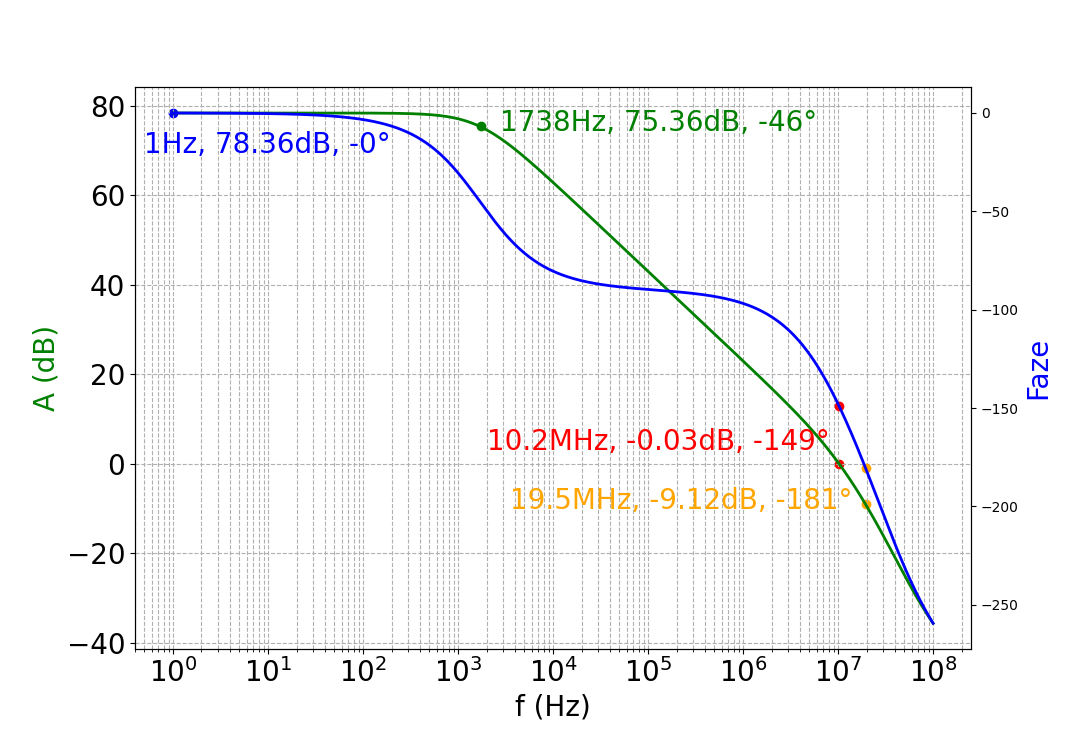
\includegraphics[width=\textwidth]{text/img/AC-charakteristika.png}
    \caption{\label{fig:res-AC-char} {\bf .AC} analýza výsledného zesilovače}
\end{figure}

Z charakteristiky \ref{fig:res-AC-char} je vidět, že stejnosměrné zesílení víc než splňuje, zesílení přes \(78 [dB]\) oproti požadovanému minimu \(60 [dB]\).

Obdobně vychází i \(GBW \approx 10.2 [MHz]\).
Přestože \(GBW\) splňuje zadání, dalo by se čekat, že bude splněno s větší rezervou vzhledem k odstupu proudu určenému splnění \(GBW\) a \(SR\).
To je pravděpodobně způsobeno zanedbáním kapacity tranzistoru \(M_7\), která tak prodlužuje časovou konstantu obvodu a tedy zmenšuje propustné pásmo.

Fázová rezerva vychází \(PM = 31^\circ\), což zadání poměrně výrazně nesplňuje.
Jak je ale vidět na časovém průběhu \ref{fig:res-TRANS-char} výstup je i přesto téměř úplně stabilní.

Amplitudová rezerva pak vychází na \(AM = -9.12 [dB]\).

Z provedené {\bf .OP} analýzy plyne hodnota offsetu \( U_{OFF} = 12 [\mu V]\), což splňuje zadání s řadovou rezervou.
Na stejném místě můžeme zjistit i spotřebu obvodu \(P_{\mathrm{diss}} = 388.8\mu \cdot 1.8 = 700 [\mu W]\).

% \begin{figure}[h!]
%     \centering
%     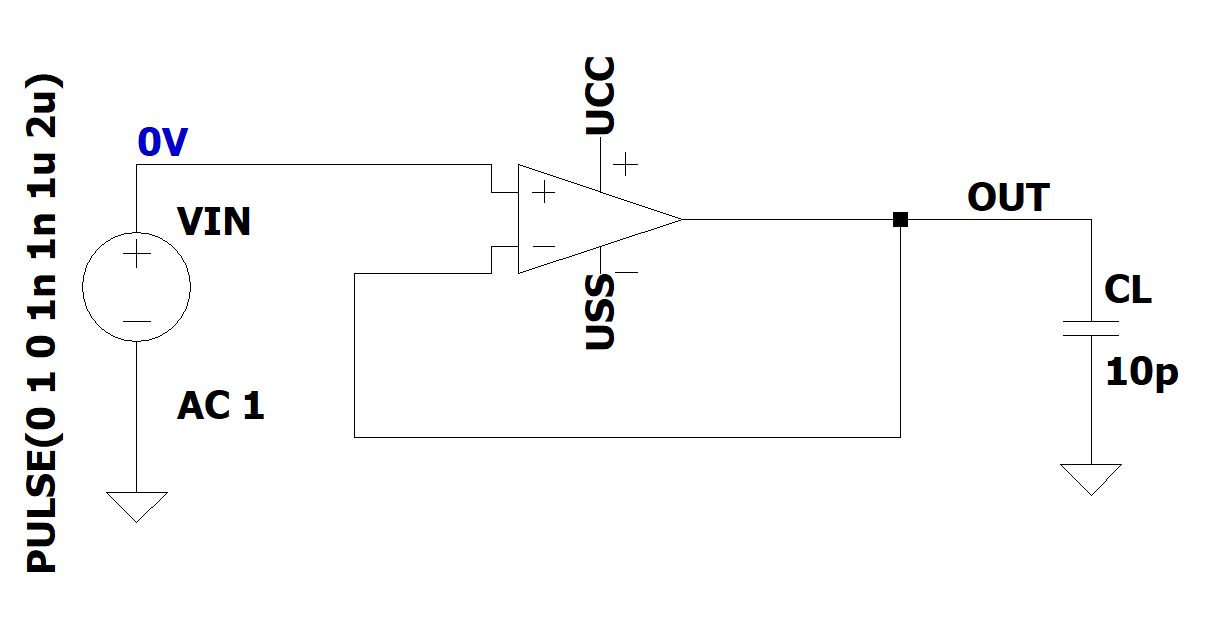
\includegraphics[width=\textwidth]{text/img/TRANS-sch.png}
%     \caption{\label{fig:res-TRANS-SCH} Zapojení zesilovače pro časovou analýzu}
% \end{figure}

\begin{figure}[h!]
    \centering
    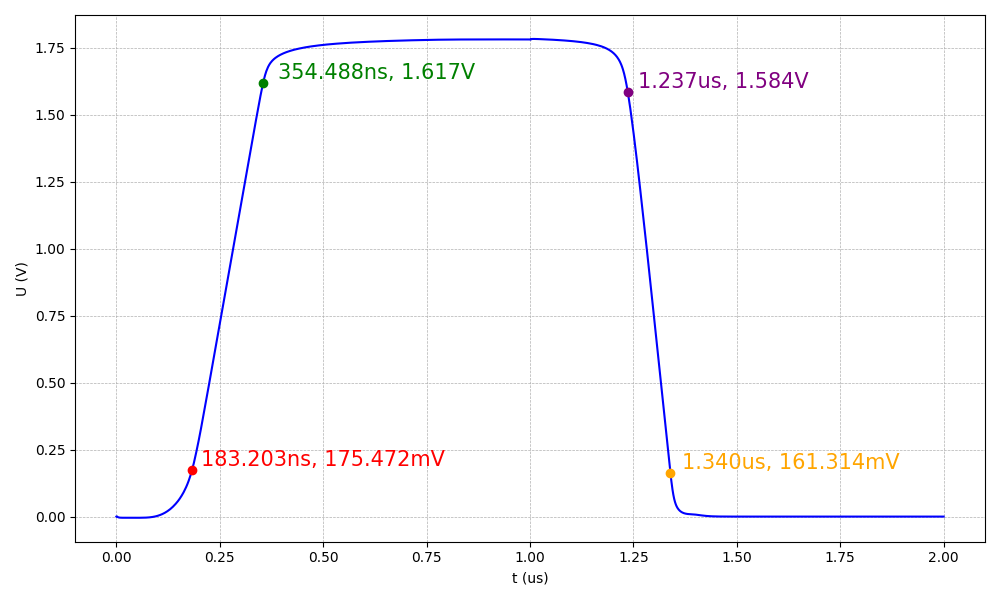
\includegraphics[width=\textwidth]{text/img/TRANS-charakteristika.png}
    \caption{\label{fig:res-TRANS-char} {\bf .TRAN} analýza výsledného zesilovače}
\end{figure}

Z průběhu na obrázku \ref{fig:res-TRANS-char} můžeme odečíst časy bodu deset devadesát pro sestupnou i vzestupnou hranu a spočítat tak \(SR\) jako:
\begin{center}
    \Large
    \(
        SR_{rise} = \frac{\Delta_U}{\Delta_t} = \frac{1.617-0.175}{354.5n - 183.2n} = 8.42 [V/\mu s]
    \)
\end{center}
\begin{center}
    \Large
    \(
        SR_{fell} = \frac{\Delta_U}{\Delta_t} = \frac{1.584 - 0.161}{1.340\mu - 1.237\mu} = 13.8 [V/\mu s]
    \)
\end{center}

Požadované \(SR\) je tedy splněné jen u sestupné hrany, kde je tranzistor \(M_7\) zavřený a celý proud \(I_{D-M6}\) je využit na vypití výstupní kapacity.

Pro určení vstupního a výstupního rozsahu budeme potřebovat dvě různá zapojení.
Zapojení pro simulaci vstupního rozsahu najdete na obrázku \ref{fig:res-DC-sch} a pro simulaci vstupního rozsahu \ref{fig:res-DC2-sch}

\begin{figure}[h!]
    \centering
    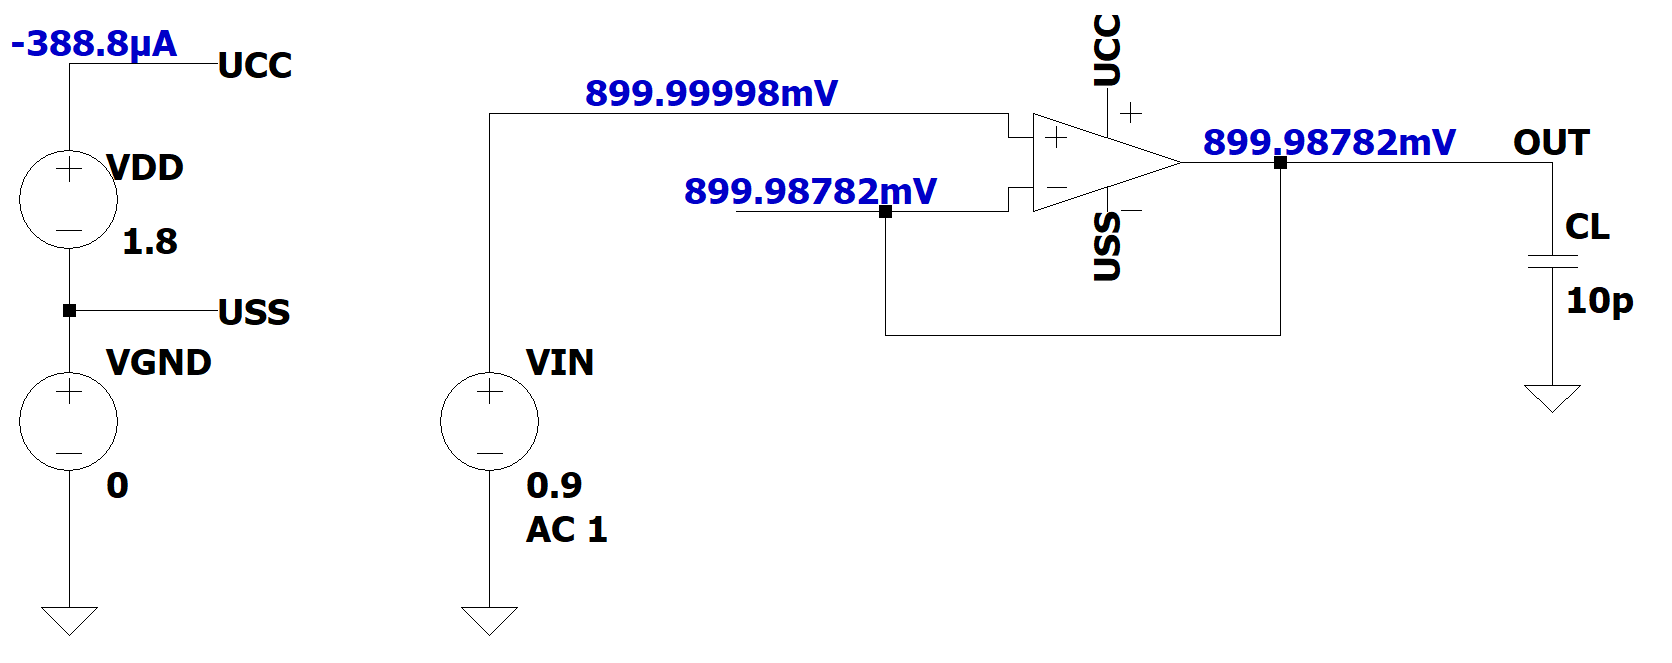
\includegraphics[width=\textwidth]{text/img/DC-sch.png}
    \caption{\label{fig:res-DC-sch} Zapojení pro {\bf .DC} analýzu vstupního rozsahu}
\end{figure}

\begin{figure}[h!]
    \centering
    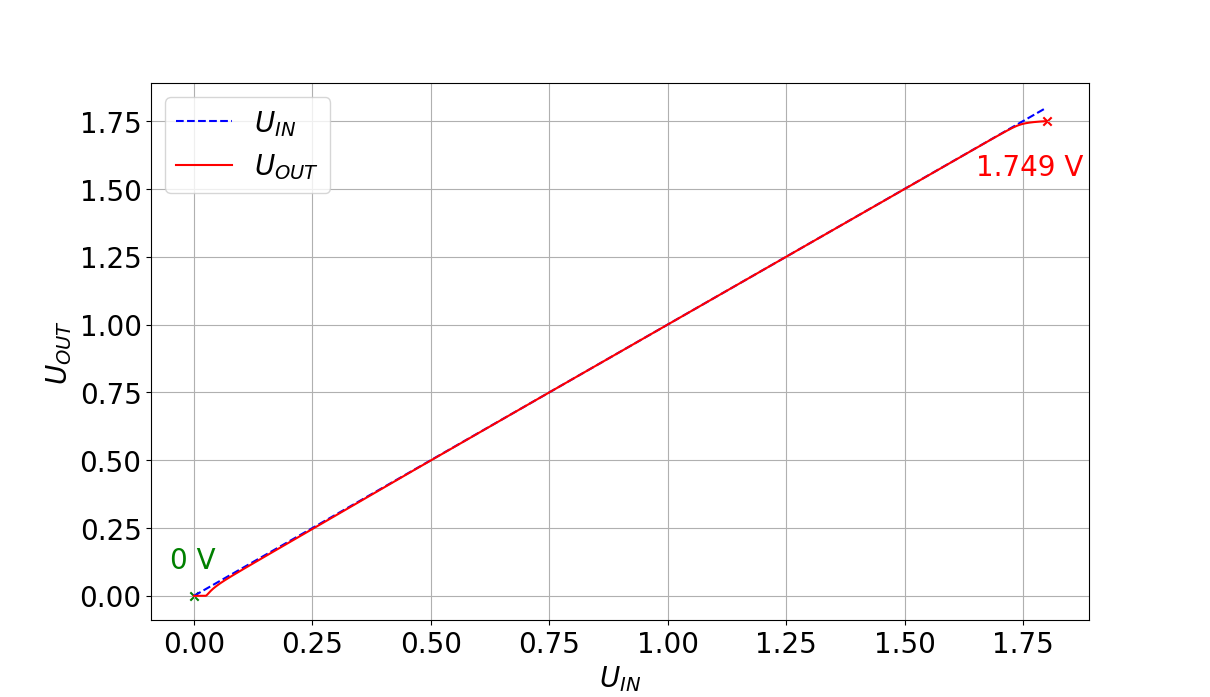
\includegraphics[width=\textwidth]{text/img/DC-charakteristika.png}
    \caption{\label{fig:res-DC-char} {\bf .DC} analýza vstupního rozsahu}
\end{figure}

\begin{figure}[h!]
    \centering
    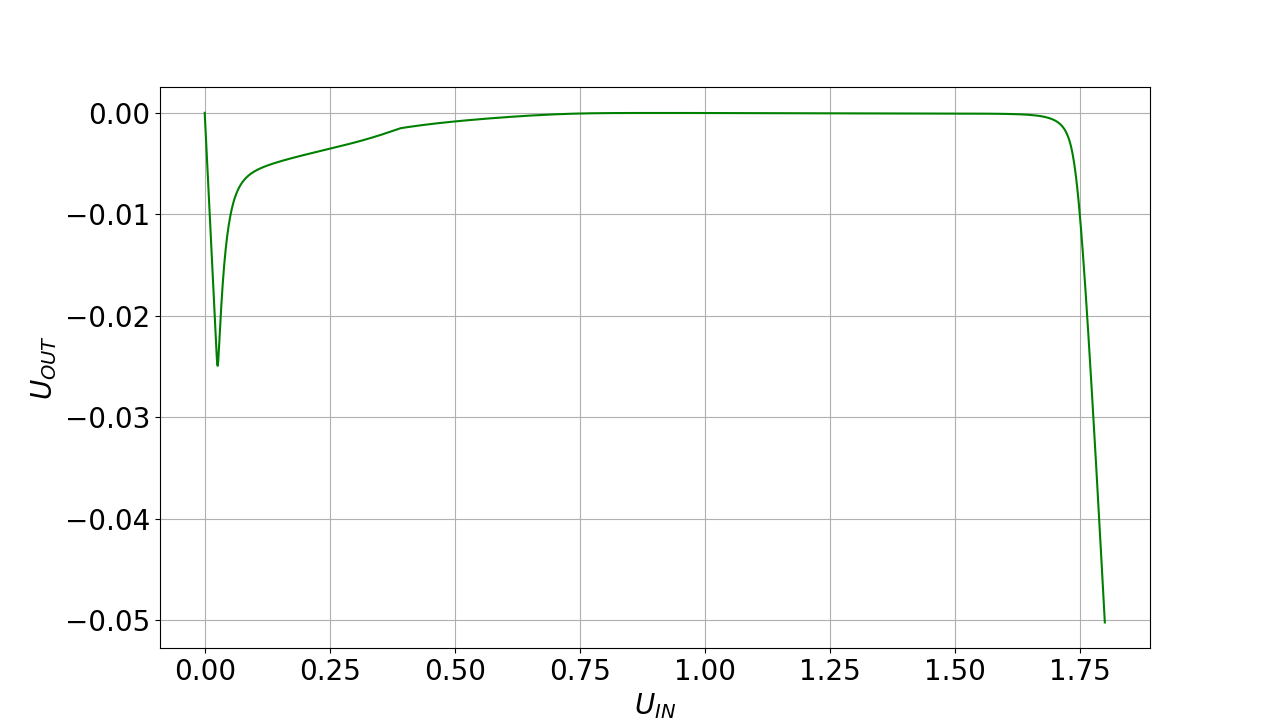
\includegraphics[width=\textwidth]{text/img/DC-korekcni.png}
    \caption{\label{fig:res-DC-korekcni} Odchylka výstupního napětí od vstupního (\(U_{IN} - U_{OUT}\)), z průběhu \ref{fig:res-DC-char}}
\end{figure}


\begin{figure}[h!]
    \centering
    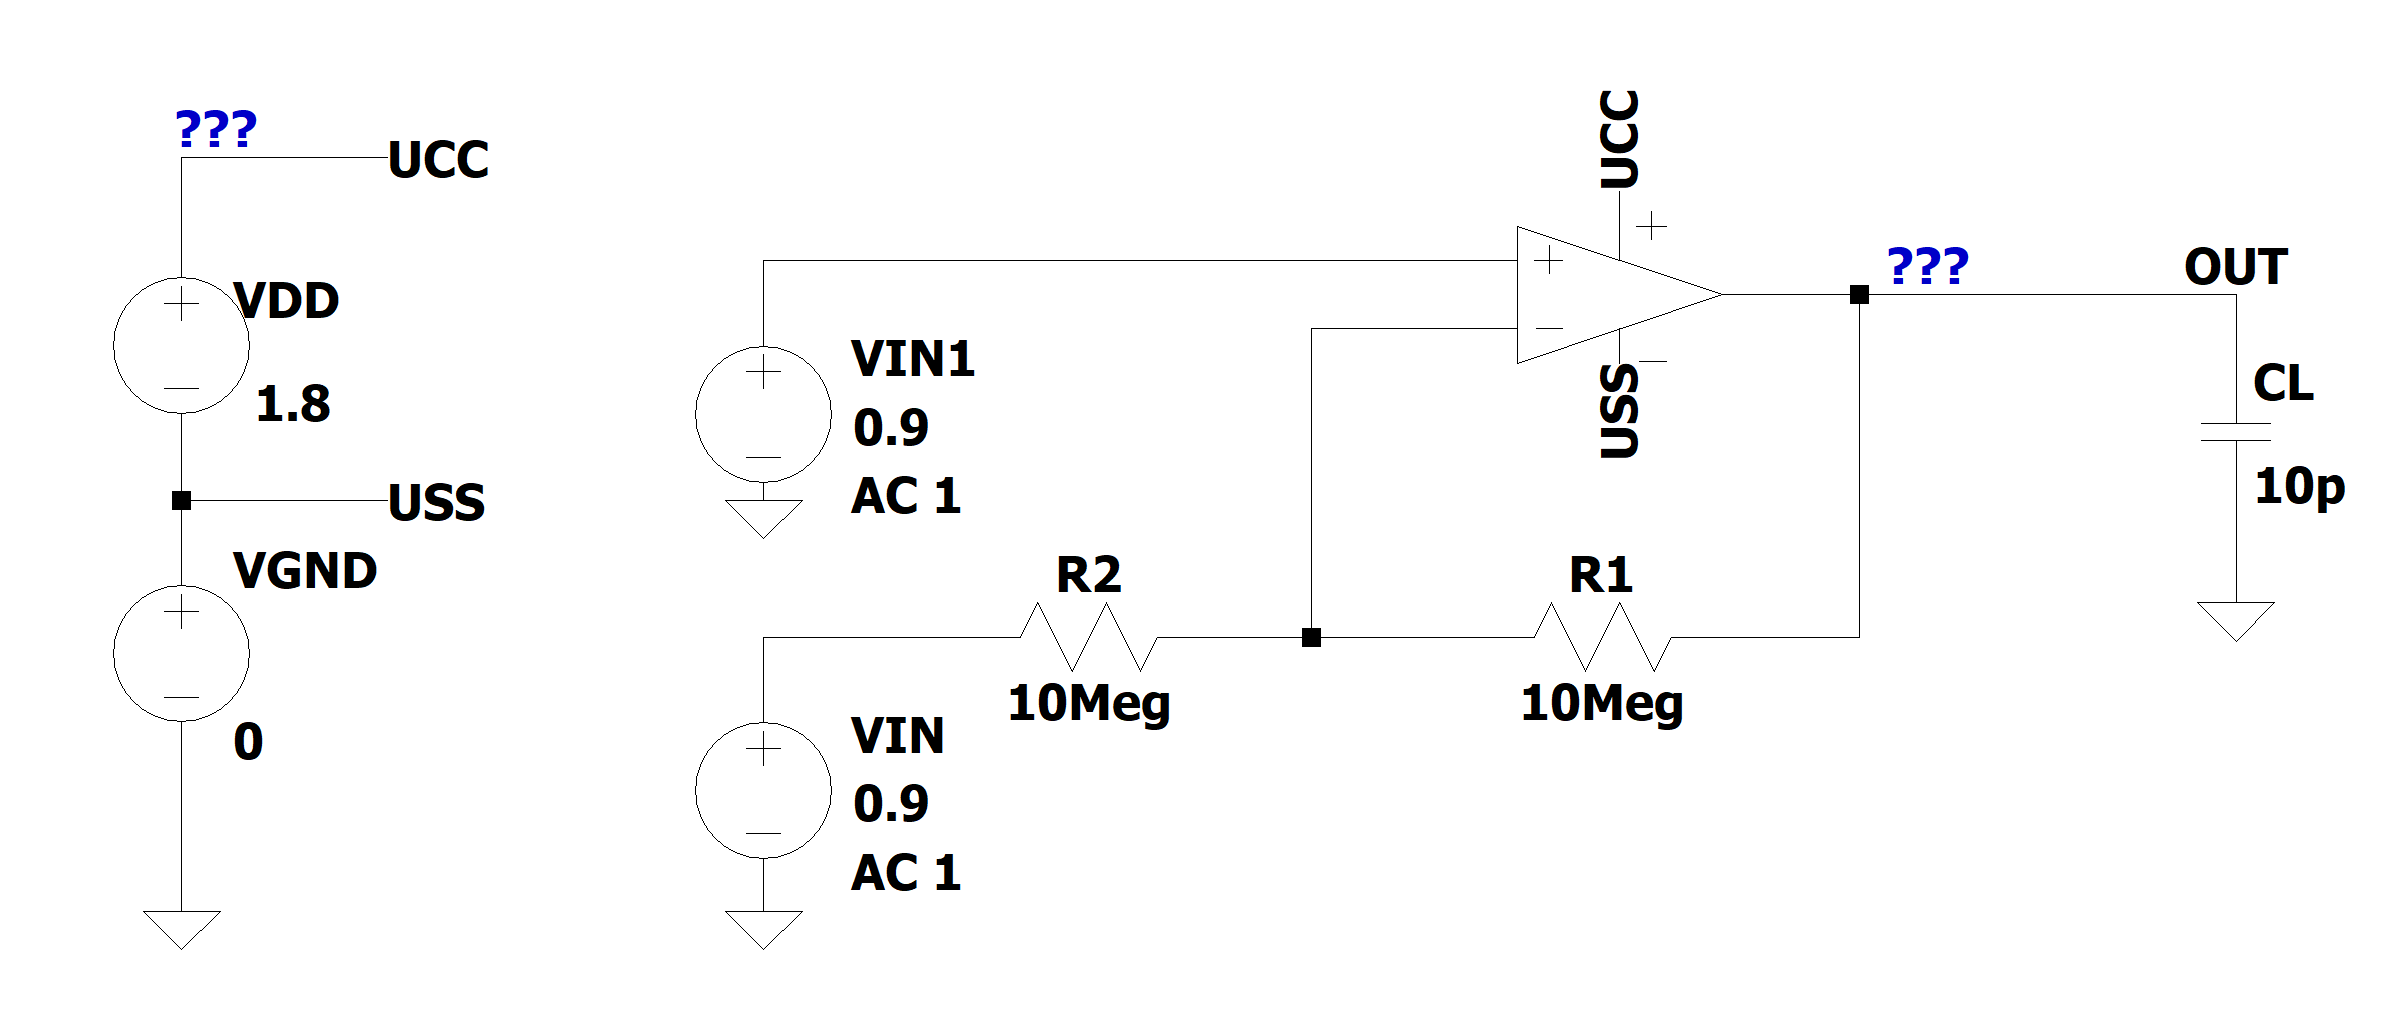
\includegraphics[width=\textwidth]{text/img/DC2-sch.png}
    \caption{\label{fig:res-DC2-sch} Zapojení pro {\bf .DC} analýzu výstupního rozsahu}
\end{figure}

\begin{figure}[h!]
    \centering
    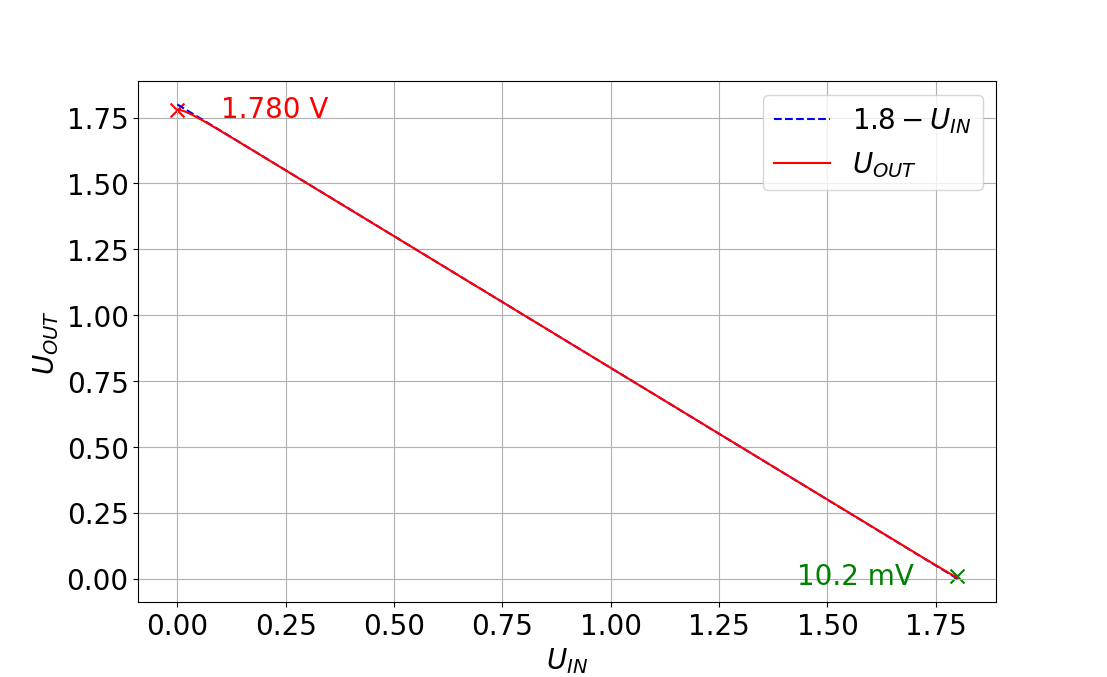
\includegraphics[width=\textwidth]{text/img/DC2-charakteristika.png}
    \caption{\label{fig:res-DC2-char} {\bf .DC} analýza výstupního rozsahu s upraveným zobrazením vstupního napětí}
\end{figure}

\begin{figure}[h!]
    \centering
    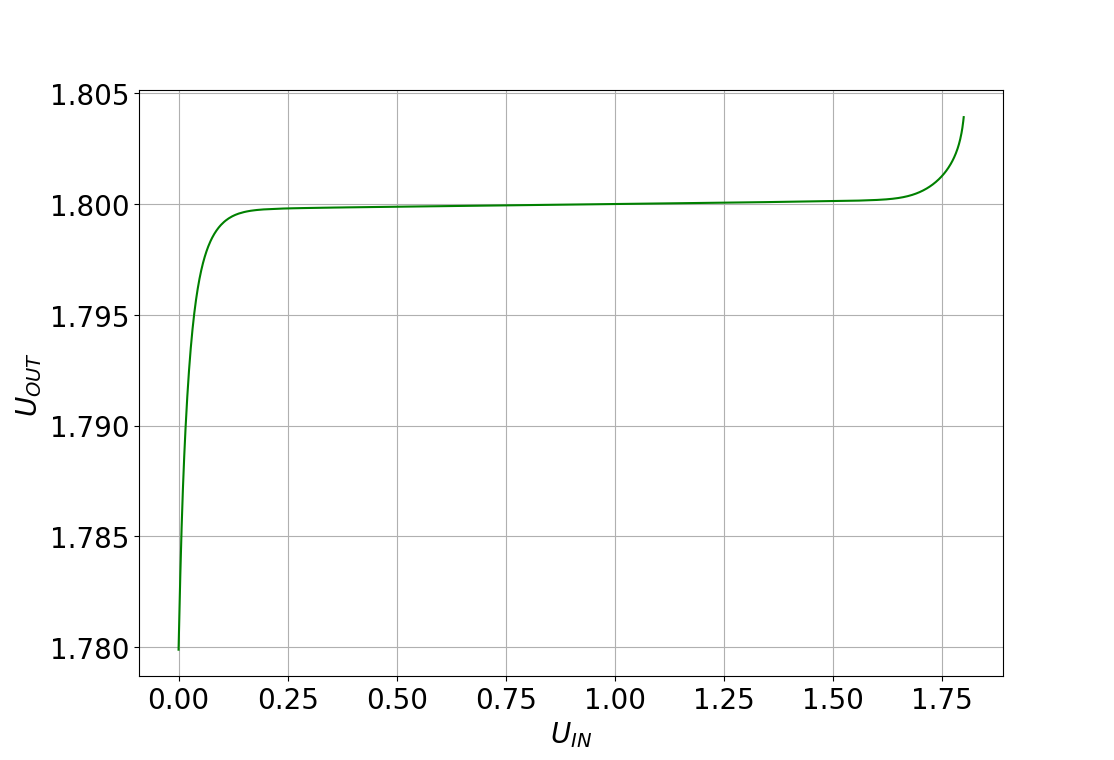
\includegraphics[width=\textwidth]{text/img/DC2-korekcni.png}
    \caption{\label{fig:res-DC2-korekcni} Odchylka výstupního napětí od vstupního (\(U_{IN} + U_{OUT}\)), z průběhu \ref{fig:res-DC2-char}}
\end{figure}

Z {\bf .DC} charakteristiky \ref{fig:res-DC-char} můžeme odečíst výstupní rozsah \($ICMR$ = 0 -> 1.749 [V]\).
Obdobně pak z {\bf .DC} charakteristiky \ref{fig:res-DC2-char} můžeme odečíst vstupní rozsah \($OVS$ = 0.01 -> 1.78 [V]\)